% !TEX root = ../main.tex
\subsection{CIFAR noisy label experiments}

Reweighting algorithm can also be useful on datasets where the labels are noisy. We study two
settings of label noise here: 
\begin{itemize}
    \vspace{-0.1in}

    \item \textsc{UniformFlip}: All label classes can uniformly flip to any other label classes,
which is the most studied in the literature.

    \vspace{-0.1in}

    \item \textsc{BackgroundFlip}: All label classes can flip to a single background class. This
noise setting is very realistic. For instance, human annotators may not have recognized all the
positive instances, while the rest remain in the background class. This is also a combination of
label imbalance and label noise since the background class usually dominates the label distribution.

\end{itemize}
We compare our method with prior work on the noisy label problem.
\vspace{-0.1in}
\begin{itemize}
\item \textsc{Reed}, proposed by \citet{reed14noisy}, is a bootstrapping technique where the
training target is a convex combination of the model prediction and the label.

\item \textsc{S-Model}, proposed by \citet{goldberger17noise}, adds a fully connected softmax layer
after the regular classification output layer to model the noise transition matrix.

\item \textsc{MentorNet}, proposed by \citet{jiang17mentornet}, is an RNN-based meta-learning model
that takes in a sequence of loss values and outputs the example weights. We compare numbers reported
in their paper with a base model that achieves similar test accuracy under 0\% noise.
\end{itemize}
In addition, we propose two simple baselines: 
1) \textsc{Random}, which assigns weights according to a rectified Gaussian (see
   Eq.~\ref{eq:randomwts});
2) \textsc{Weighted}, designed for \textsc{BackgroundFlip}, where the model
knows the oracle noise ratio for each class and reweights the training loss proportional to the
percentage of clean images of that label class.
\vspace{-0.05in}
\paragraph{Clean validation set} For \textsc{UniformFlip}, we use 1,000 clean images in the
validation set; for \textsc{BackgroundFlip}, we use 10 clean images per label class. Since our
method uses information from the clean validation, for a fair comparison, we conduct an additional
finetuning on the clean data based on the pre-trained baselines. We also study the effect on the
size of the clean validation set in an ablation study.
\vspace{-0.05in}
\paragraph{Hyper-validation set} For monitoring training progress and tuning baseline
hyperparameters, we split out another 5,000 hyper-validation set from the 50,000 training images. We
also corrupt the hyper-validation set with the same noise type.
% !TEX root = ../main.tex

\begin{table}[t]
\begin{center}
\caption{CIFAR \textsc{UniformFlip} under 40\% noise ratio using a WideResNet-28-10 model. Test
accuracy shown in percentage. Top rows use only noisy data, and bottom uses additional 1000 clean
images. ``FT'' denotes fine-tuning on clean data.}
\label{tab:uniformflip}
\vskip 0.1in
\begin{small}
\begin{sc}
\begin{tabular}{ccc}
\toprule
Model              &  CIFAR-10                    & CIFAR-100                     \\
\midrule
Baseline           & 67.97 $\pm$ 0.62             & 50.66 $\pm$ 0.24              \\
Reed-Hard          & 69.66 $\pm$ 1.21             & 51.34 $\pm$  0.17             \\
S-Model            & 70.64 $\pm$ 3.09             & 49.10 $\pm$ 0.58              \\
MentorNet          & 76.6                         & 56.9                          \\
Random             & 86.06 $\pm$ 0.32.            & 58.01 $\pm$ 0.37              \\
\midrule
\multicolumn{3}{c}{Using 1,000 clean images} \\
\midrule
Clean Only         & 46.64 $\pm$ 3.90             & 9.94 $\pm$ 0.82               \\
Baseline +FT       & 78.66 $\pm$ 0.44             & 54.52 $\pm$ 0.40              \\
MentorNet +FT      & 78                           & 59                            \\
Random +FT         & 86.55 $\pm$ 0.24             & 58.54 $\pm$ 0.52              \\
Ours               & \textbf{86.92 $\pm$ 0.19}    & \textbf{61.34 $\pm$ 2.06}     \\
\bottomrule
\end{tabular}
\end{sc}
\end{small}
\end{center}
\vskip -0.1in
\end{table}
% !TEX root = ../main.tex

\begin{table}[t]
\begin{center}

\caption{CIFAR \textsc{BackgroundFlip} under 40\% noise ratio using a ResNet-32 model. Test accuracy
shown in percentage. Top rows use only noisy data, and bottom rows use additional 10 clean images
per class. ``+ES'' denotes early stopping; ``FT'' denotes fine-tuning.}

\label{tab:backgroundflip}

\resizebox{\columnwidth}{!}{
\begin{small}
\begin{sc}
\begin{tabular}{ccc}
\toprule
Model                             & CIFAR-10                    & CIFAR-100                     \\
\midrule
Baseline                          & 59.54 $\pm$ 2.16            & 37.82 $\pm$ 0.69              \\
Baseline +ES                      & 64.96 $\pm$ 1.19            & 39.08 $\pm$ 0.65              \\
Random                            & 69.51 $\pm$ 1.36            & 36.56 $\pm$ 0.44              \\
Weighted                          & 79.17 $\pm$ 1.36            & 36.56 $\pm$ 0.44              \\
Reed Soft +ES                     & 63.47 $\pm$ 1.05            & 38.44 $\pm$ 0.90              \\
Reed Hard +ES                     & 65.22 $\pm$ 1.06            & 39.03 $\pm$ 0.55              \\
S-Model                           & 58.60 $\pm$ 2.33            & 37.02 $\pm$ 0.34              \\
S-Model +Conf                     & 68.93 $\pm$ 1.09            & 46.72 $\pm$ 1.87              \\
S-Model +Conf +ES                 & 79.24 $\pm$ 0.56            & 54.50 $\pm$ 2.51              \\
\midrule
\multicolumn{3}{c}{Using 10 clean images per class} \\
\midrule
Clean Only                        & 15.90 $\pm$ 3.32            & 8.06  $\pm$ 0.76              \\
Baseline +FT                      & 82.82 $\pm$ 0.93            & 54.23 $\pm$ 1.75              \\
Baseline +ES +FT                  & 85.19 $\pm$ 0.46            & 55.22 $\pm$ 1.40              \\
Weighted +FT                      & 85.98 $\pm$ 0.47            & 53.99 $\pm$ 1.62              \\
S-Model +Conf +FT                 & 81.90 $\pm$ 0.85            & 53.11 $\pm$ 1.33              \\
S-Model +Conf +ES +FT             & 85.86 $\pm$ 0.63            & 55.75 $\pm$ 1.26              \\
Ours                              & \textbf{86.73 $\pm$ 0.48}   & \textbf{59.30 $\pm$ 0.60}     \\
\bottomrule
\end{tabular}
\end{sc}
\end{small}
}
\end{center}
\vskip -0.1in
\end{table}
\vspace{-0.05in}
\paragraph{Experimental details} For \textsc{Reed} model, we use the best $\beta$ reported in
\citet{reed14noisy} ($\beta=0.8$ for hard bootstrapping and $\beta=0.95$ for soft bootstrapping).
For the \textsc{S-Model}, we explore two versions to initialize the transition weights: 1) a
smoothed identity matrix; 2) in background flip experiments we consider initializing the transition
matrix with the confusion matrix of a pre-trained baseline model (\textsc{S-Model +Conf}). We find
baselines can easily overfit the training noise, and therefore we also study early stopped versions
of the baselines to provide a stronger comparison. In contrast, we find early stopping not necessary
for our method.

To make our results comparable with the ones reported in \textsc{MentorNet} and to save computation
time, we exchange their Wide ResNet-101-10 with a Wide ResNet-28-10 (WRN-28-10) \cite{wrn} with
dropout 0.3 as our base model in the \textsc{UniformFlip} experiments. We find that test accuracy
differences between the two base models are within 0.5\% on CIFAR datasets under 0\% noise. In the
\textsc{BackgroundFlip} experiments, we use a ResNet-32 \cite{resnet} as our base model.

We train the models with SGD with momentum, at an initial learning rate 0.1 and a momentum 0.9 with
mini-batch size 100. For ResNet-32 models, the learning rate decays $\times 0.1$ at 40K and 60K
steps, for a total of 80K steps. For WRN and early stopped versions of ResNet-32 models, the
learning rate decays at 40K and 50K steps, for a total of 60K steps. Under regular 0\% noise
settings, our base ResNet-32 gets 92.5\% and 68.1\% classification accuracy on CIFAR-10 and 100, and
the WRN-28-10 gets 95.5\% and 78.2\%. For the finetuning stage, we run extra 5K steps of training on
the limited clean data.

We report the average test accuracy for 5 different random splits of clean and noisy labels, with
95\% confidence interval in Table~\ref{tab:uniformflip} and \ref{tab:backgroundflip}. The background
classes for the 5 trials are [0, 1, 3, 5, 7] (CIFAR-10) and [7, 12, 41, 62, 85] (CIFAR-100).

% !TEX root = ../main.tex
\begin{figure}[t]
\centering
\iflatexml
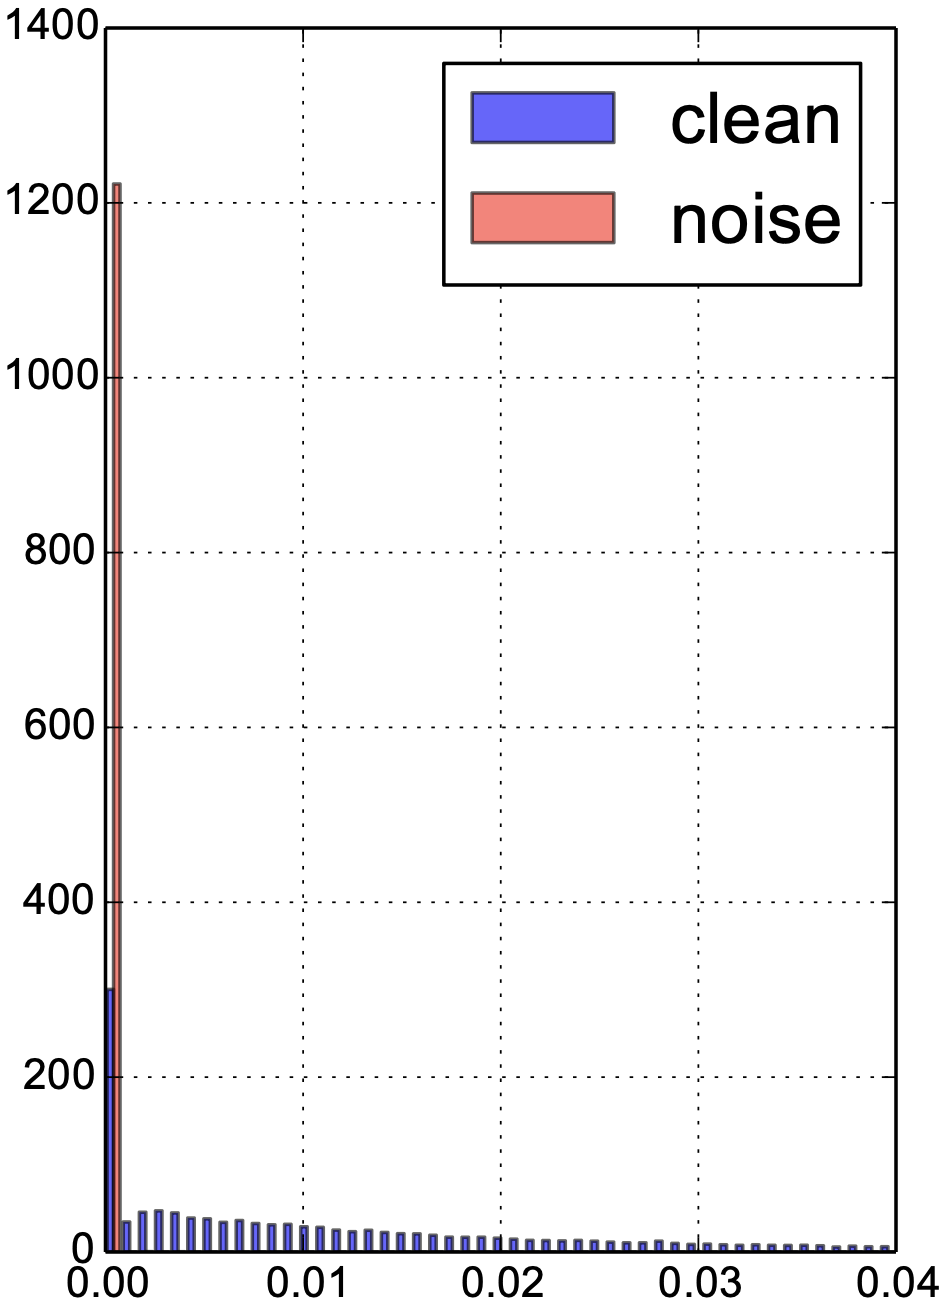
\includegraphics[width=3\columnwidth]{figures/uncondition.png}
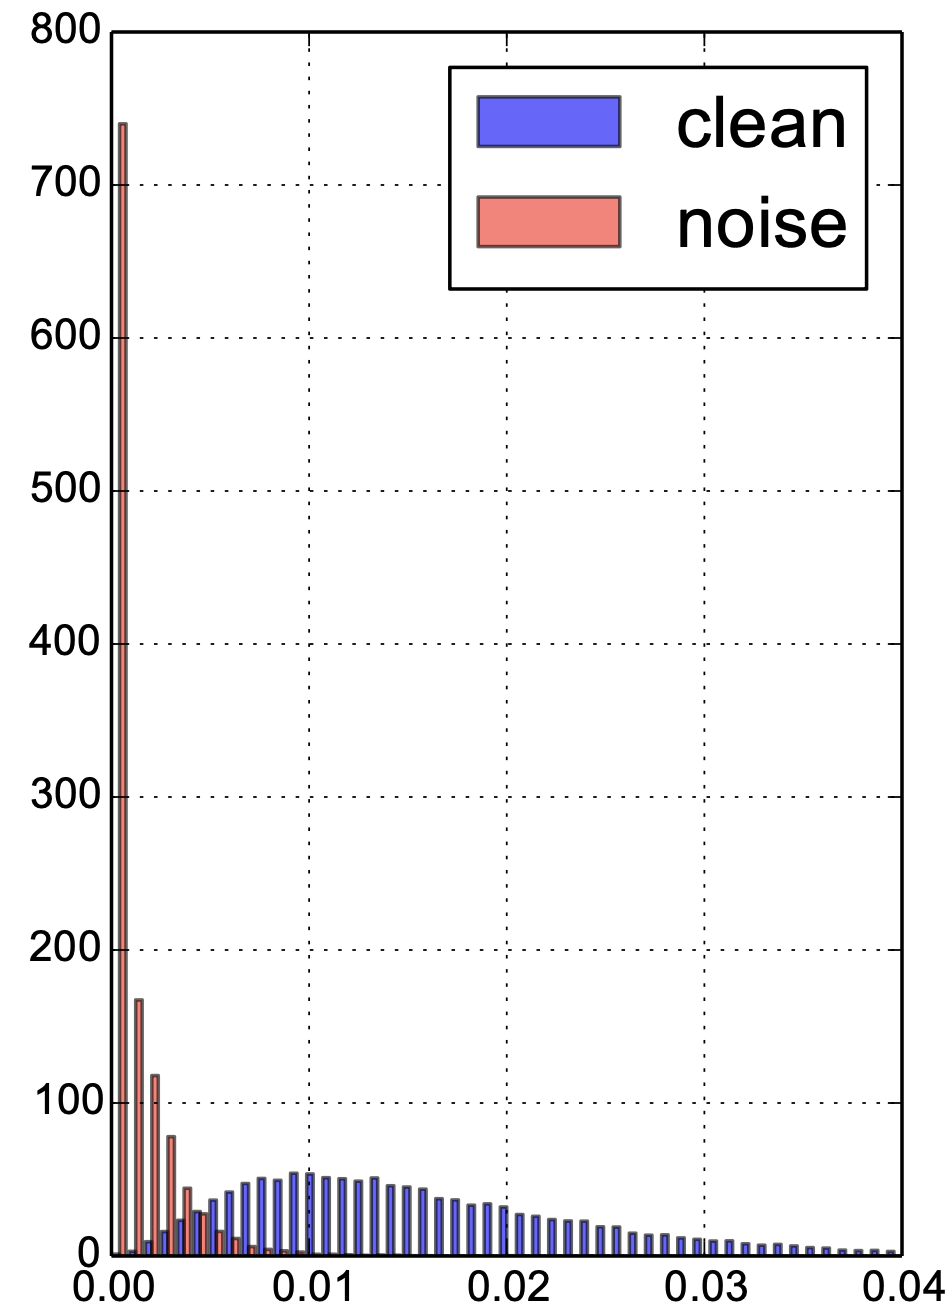
\includegraphics[width=3\columnwidth]{figures/condition.png}
\else
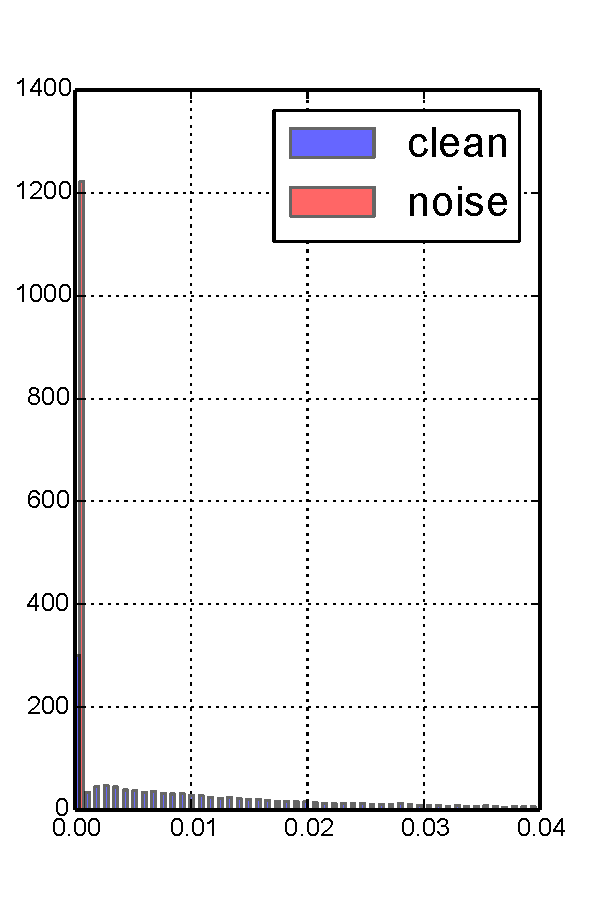
\includegraphics[width=0.45\columnwidth,trim={0cm 0 0cm 0},clip]{figures/uncondition.pdf}
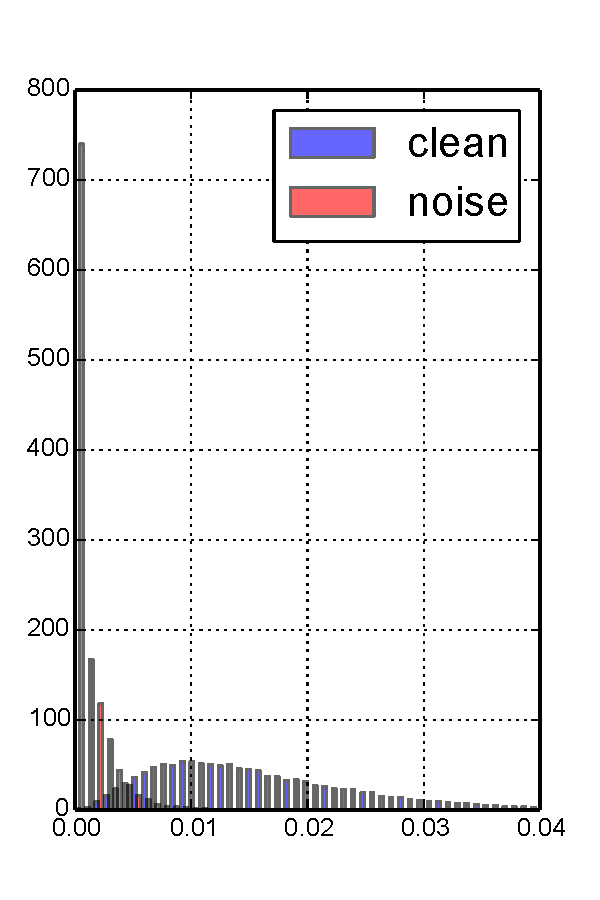
\includegraphics[width=0.45\columnwidth,trim={0cm 0 0cm 0},clip]{figures/condition.pdf}
\fi
\vspace{-0.1in}
\caption{Example weights distribution on \textsc{BackgroundFlip}. Left: a hyper-validation batch,
with randomly flipped background noises. Right: a hyper-validation batch containing only on a single
label class, with flipped background noises, averaged across all non-background classes.}
\label{fig:dist}
\end{figure}

% !TEX root = ../main.tex

\begin{figure}[t]
\centering
\iflatexml
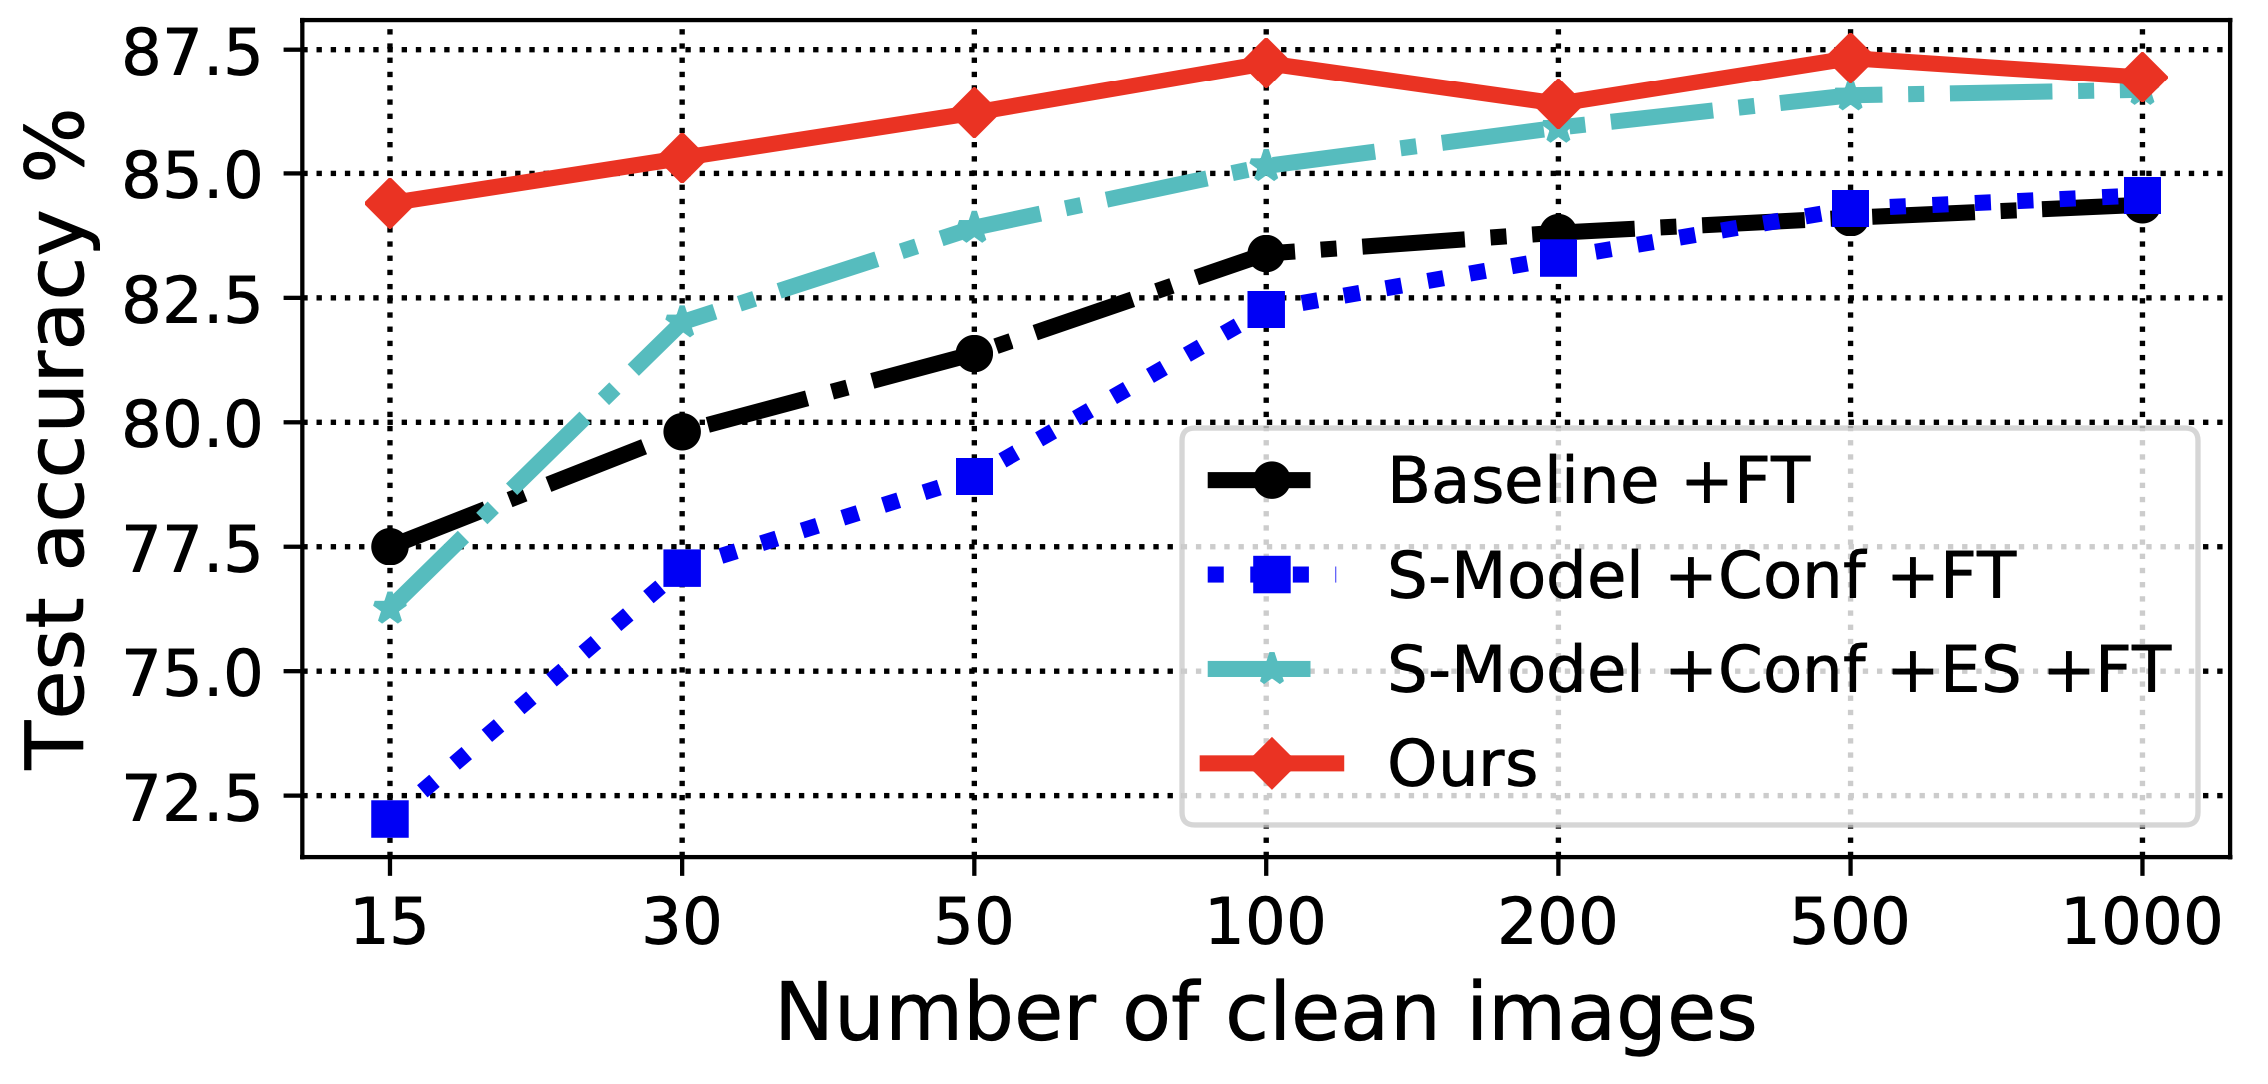
\includegraphics[width=6\columnwidth]{figures/cifar-imbalance-ft.png}
\else
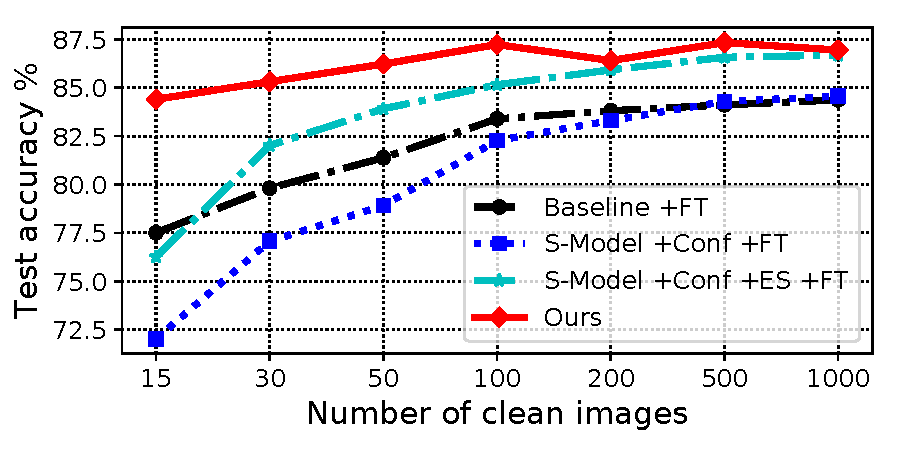
\includegraphics[width=0.9\columnwidth]{figures/cifar-imbalance-ft.pdf}
\fi
\vspace{-0.1in}
\caption{Effect of the number of clean imaged used, on CIFAR-10 with 40\% of data flipped to label 3. ``ES'' denotes early stopping.}
\label{fig:ft}
\end{figure}

% !TEX root = ../main.tex

\begin{figure}[t]
\centering
\iflatexml
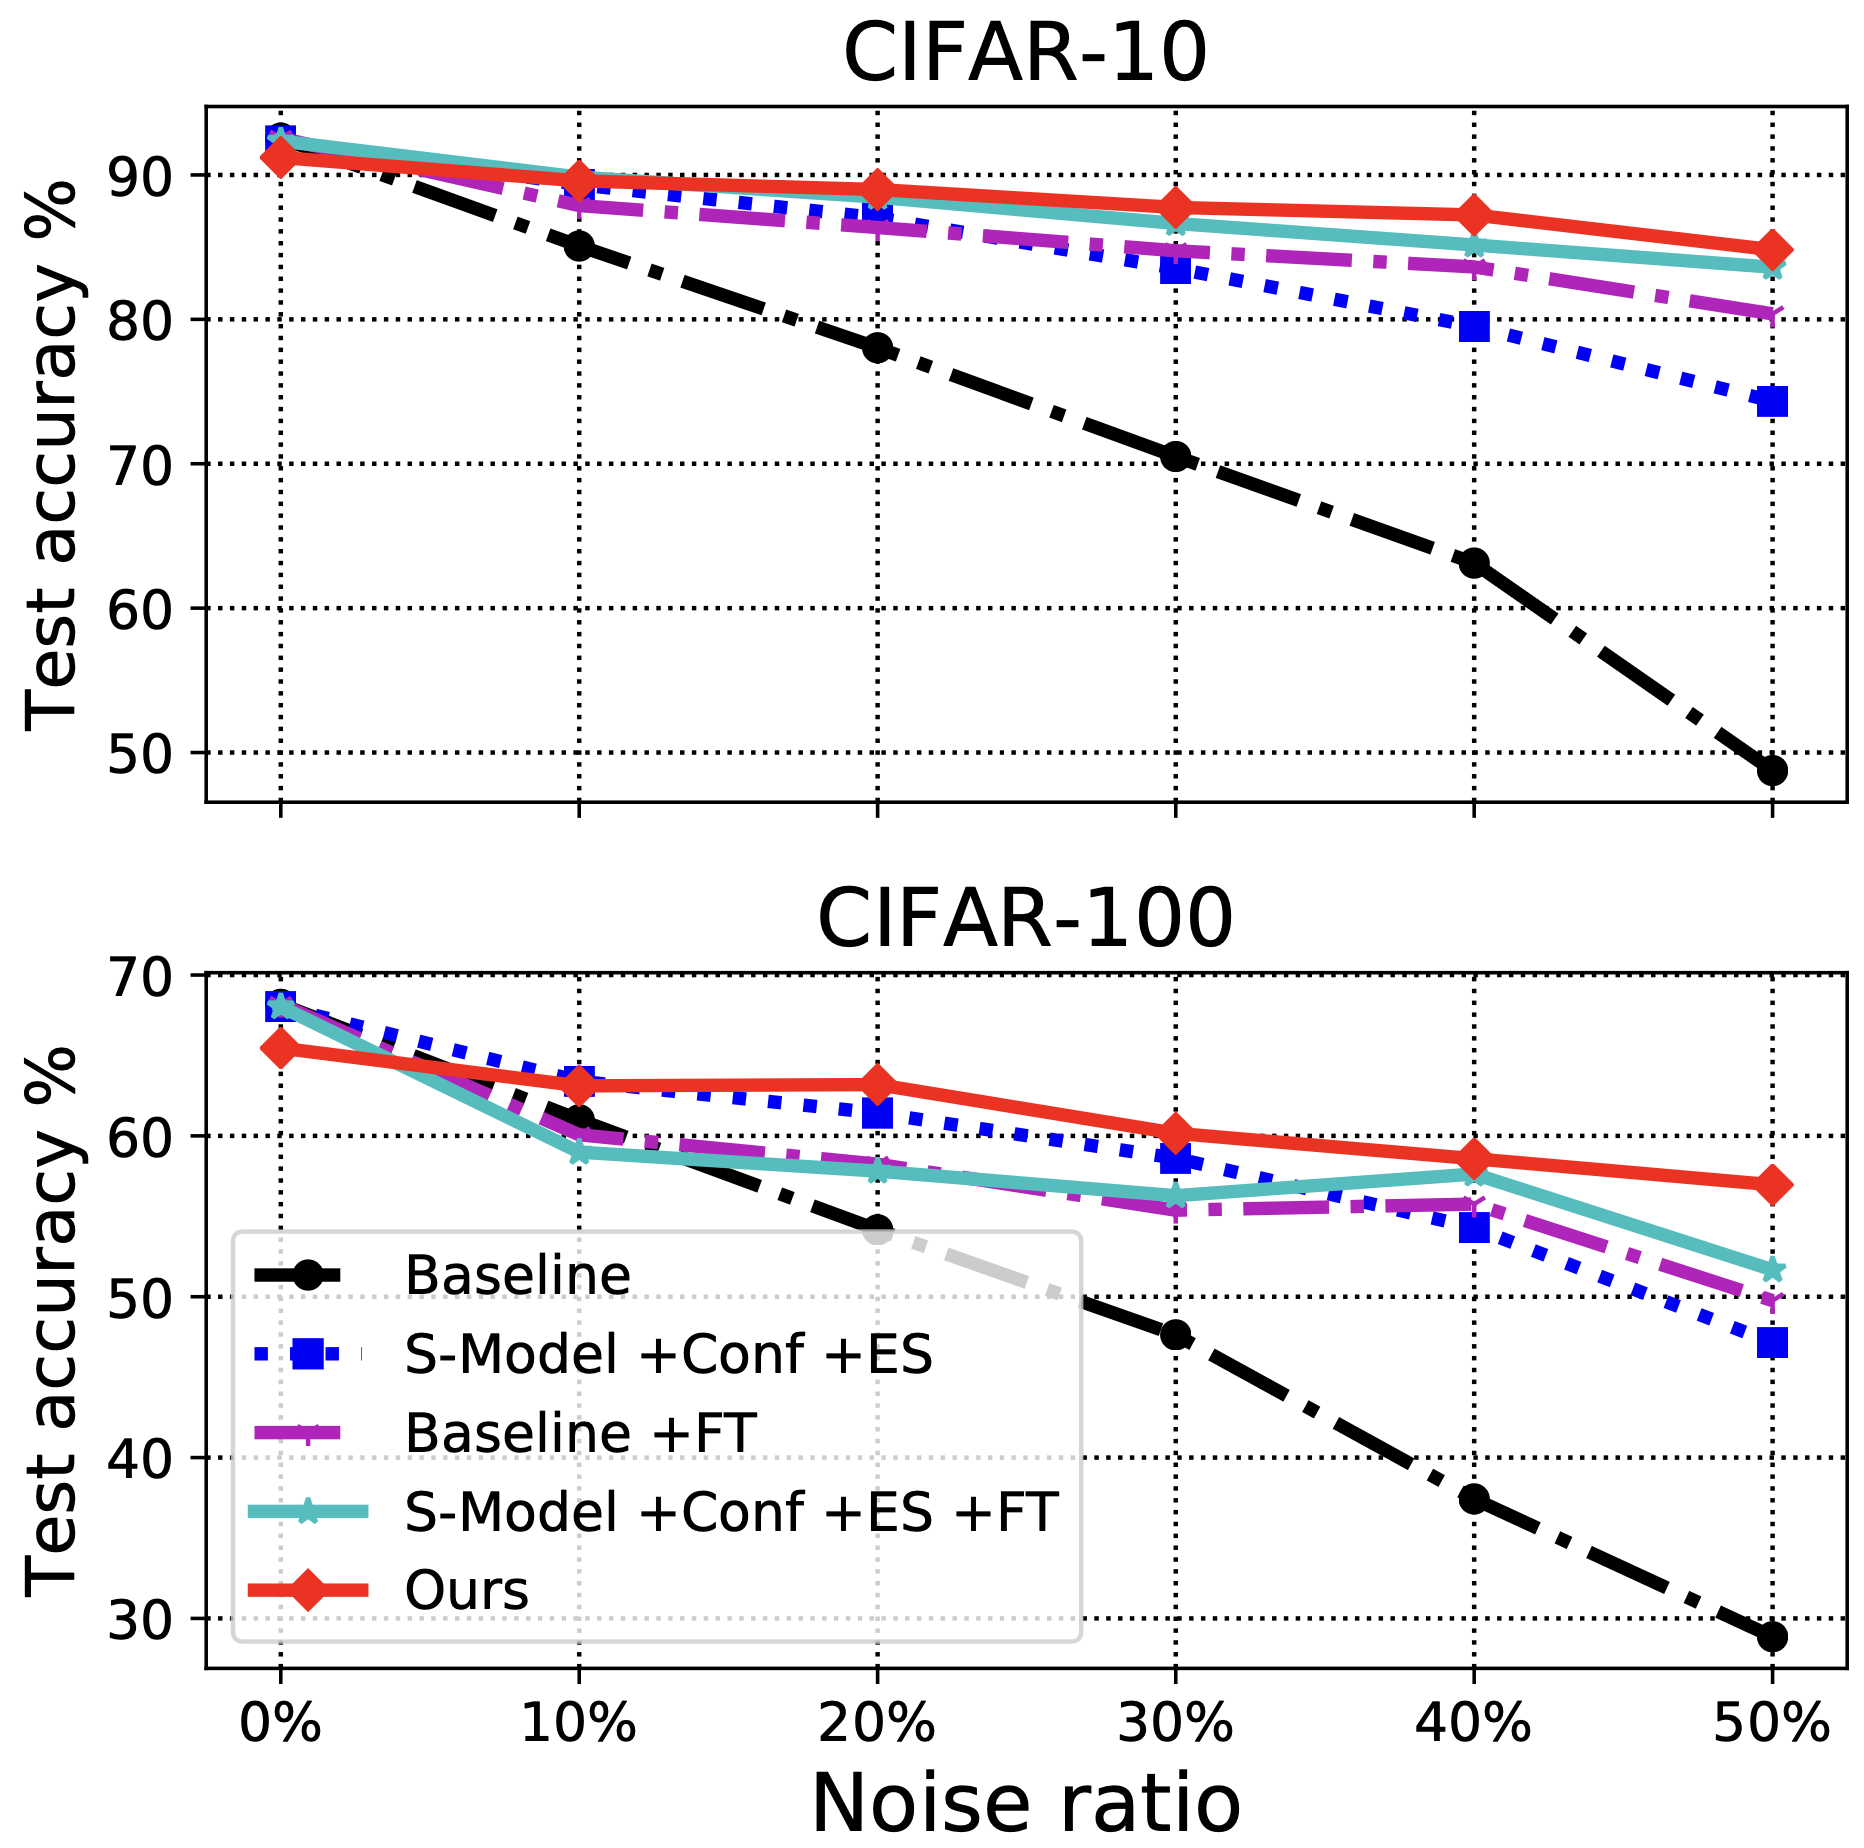
\includegraphics[width=6\columnwidth]{figures/cifar-noisy-imbalance-level.png}
\else
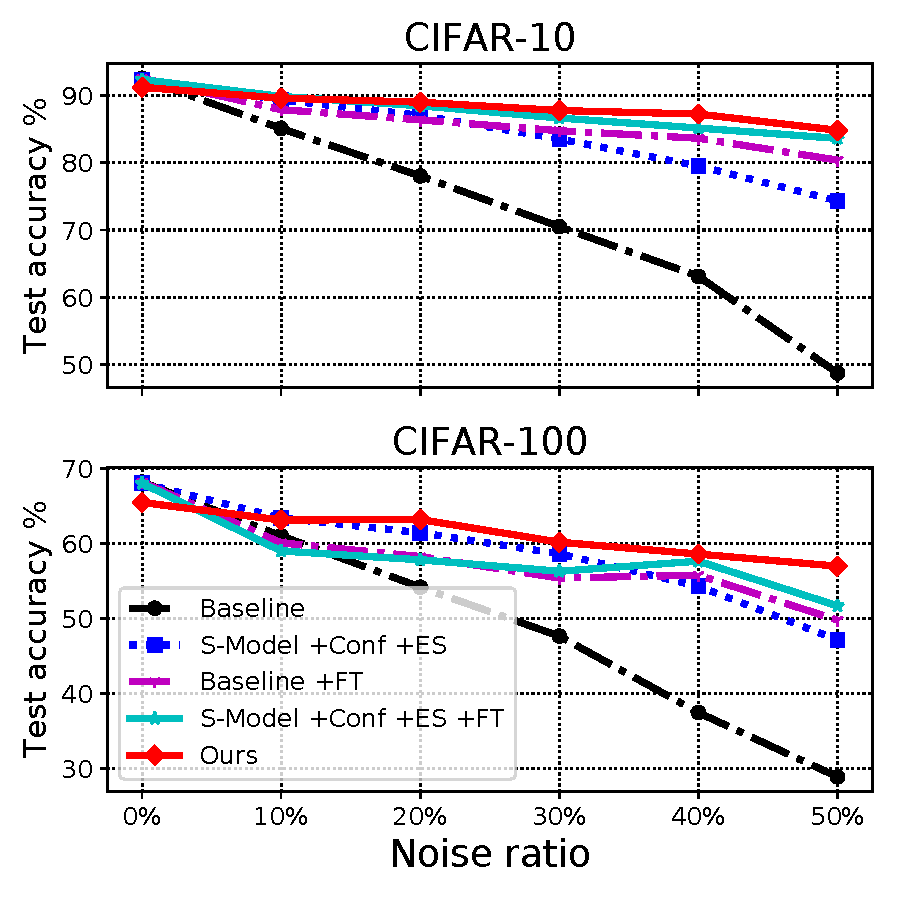
\includegraphics[width=0.9\columnwidth]{figures/cifar-noisy-imbalance-level.pdf}
\fi
\vspace{-0.1in}

\caption{Model test accuracy on imbalanced noisy CIFAR experiments across various noise levels using
a base ResNet-32 model. ``ES'' denotes early stopping, and ``FT'' denotes finetuning.}
\label{fig:level}

\end{figure}

% !TEX root = ../main.tex
\begin{figure}[h!]
\centering
\vspace{-0.1in}
\iflatexml
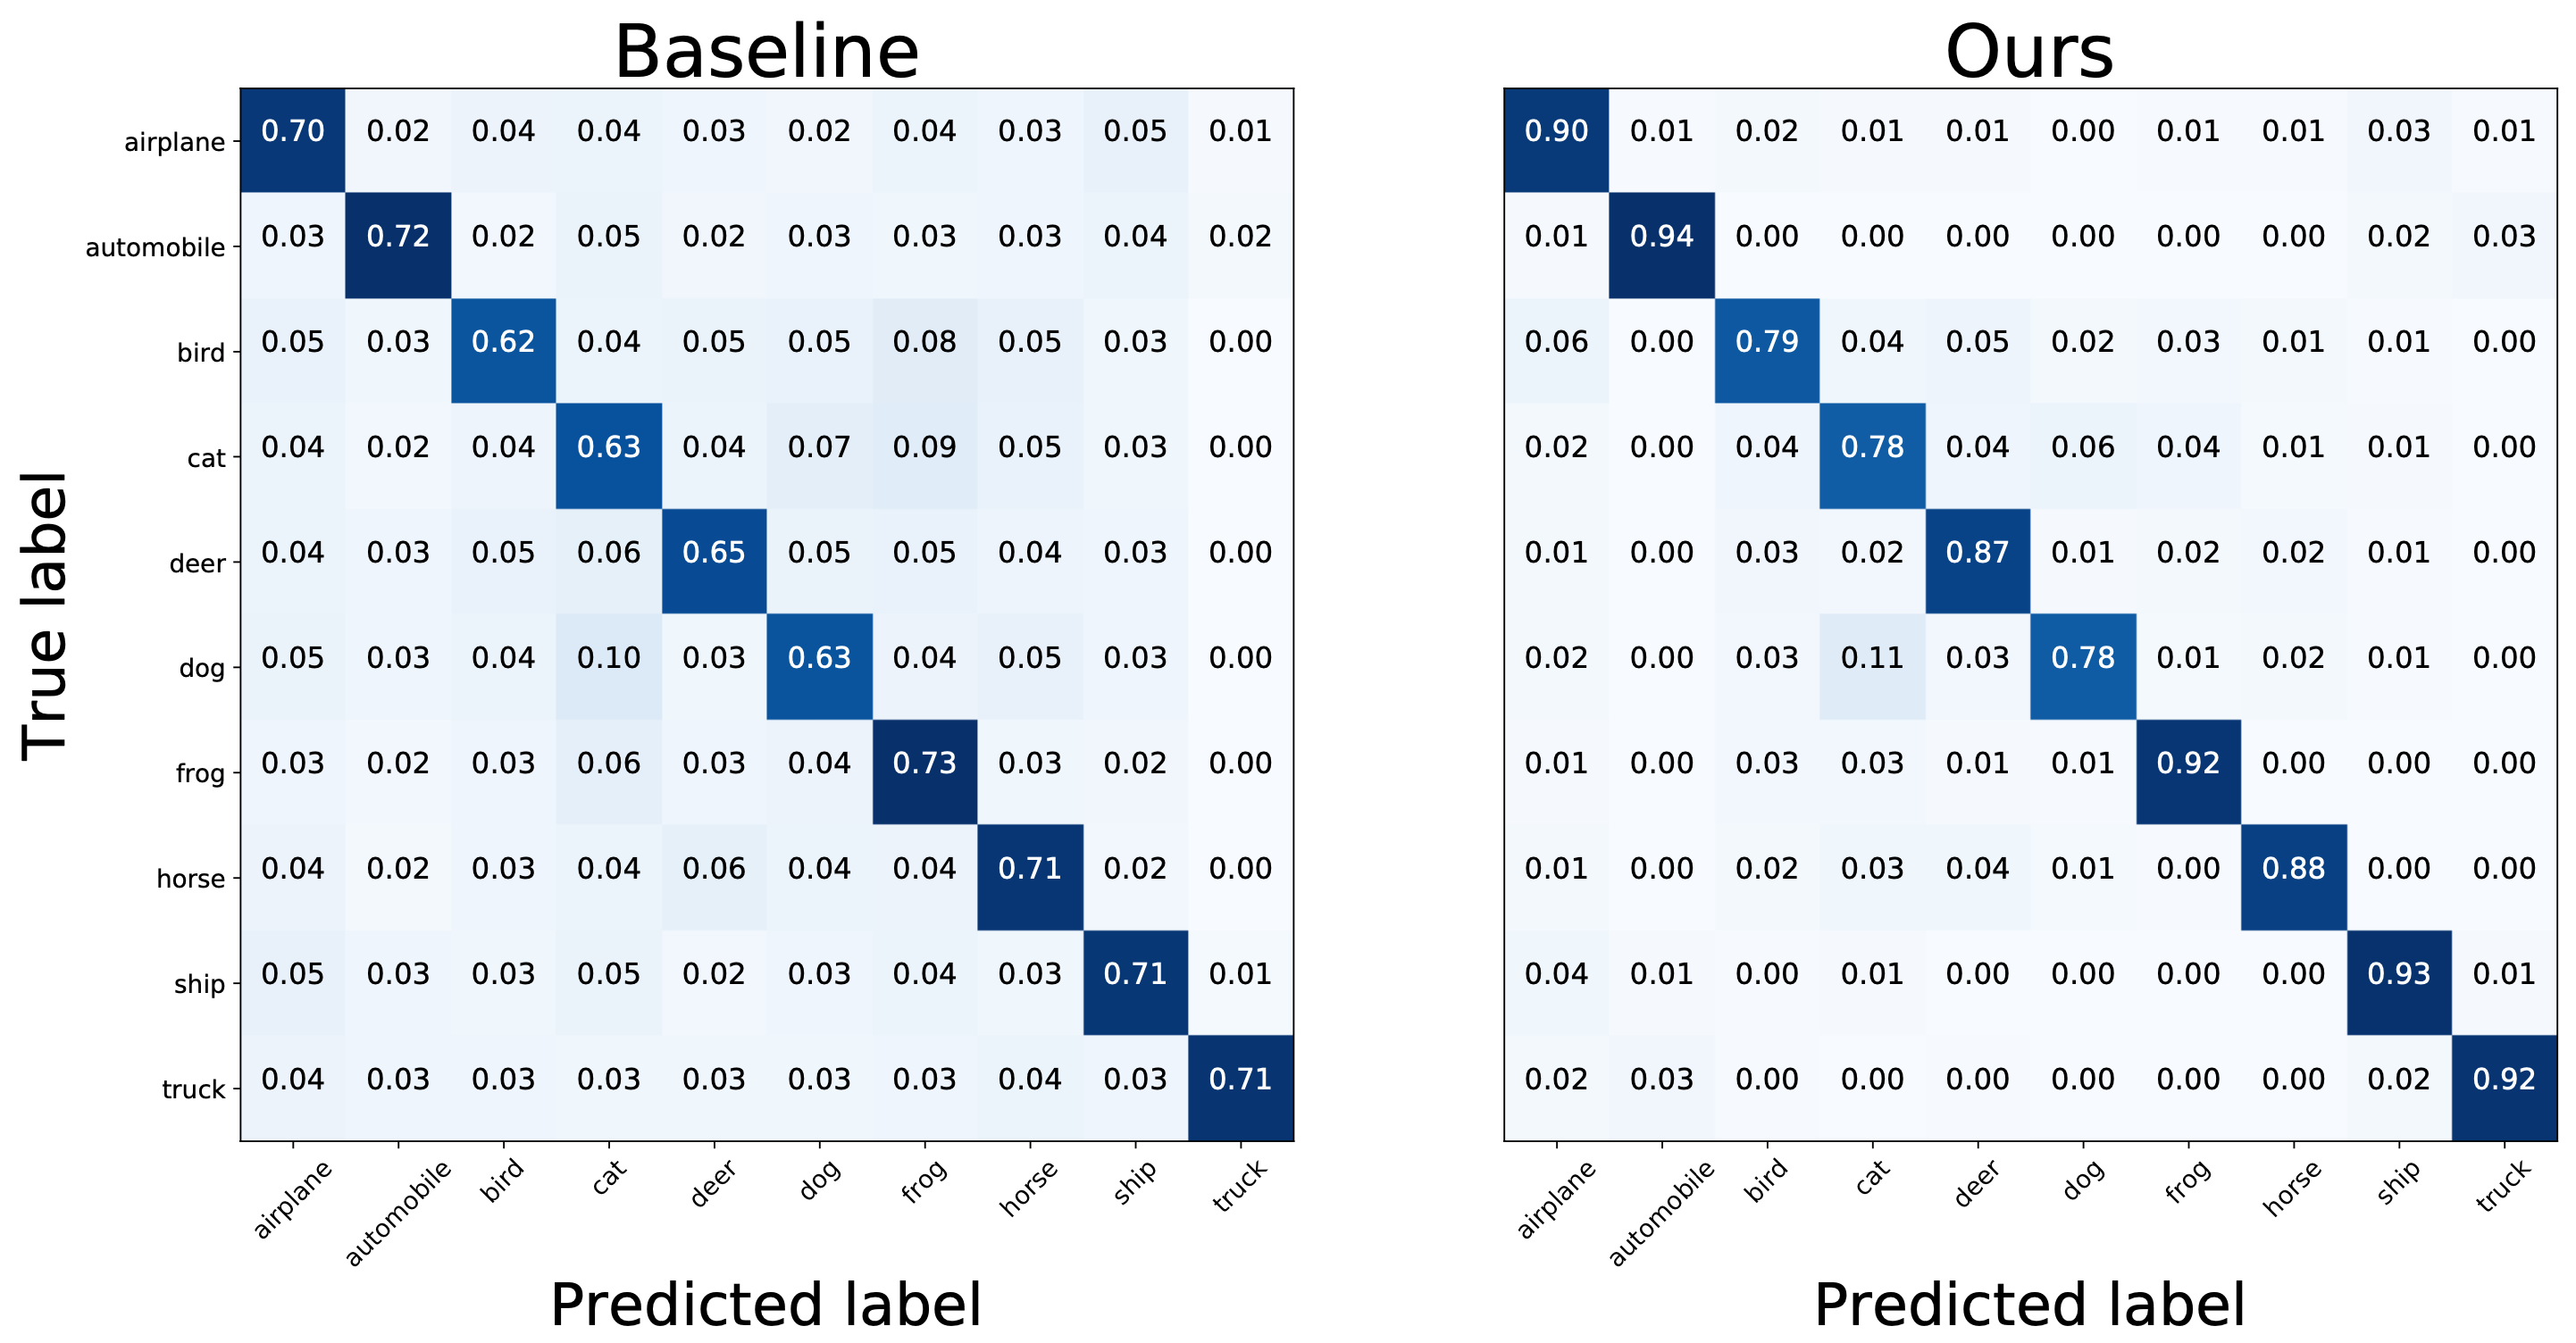
\includegraphics[width=3\columnwidth]{figures/cifar-noise-cm.png}
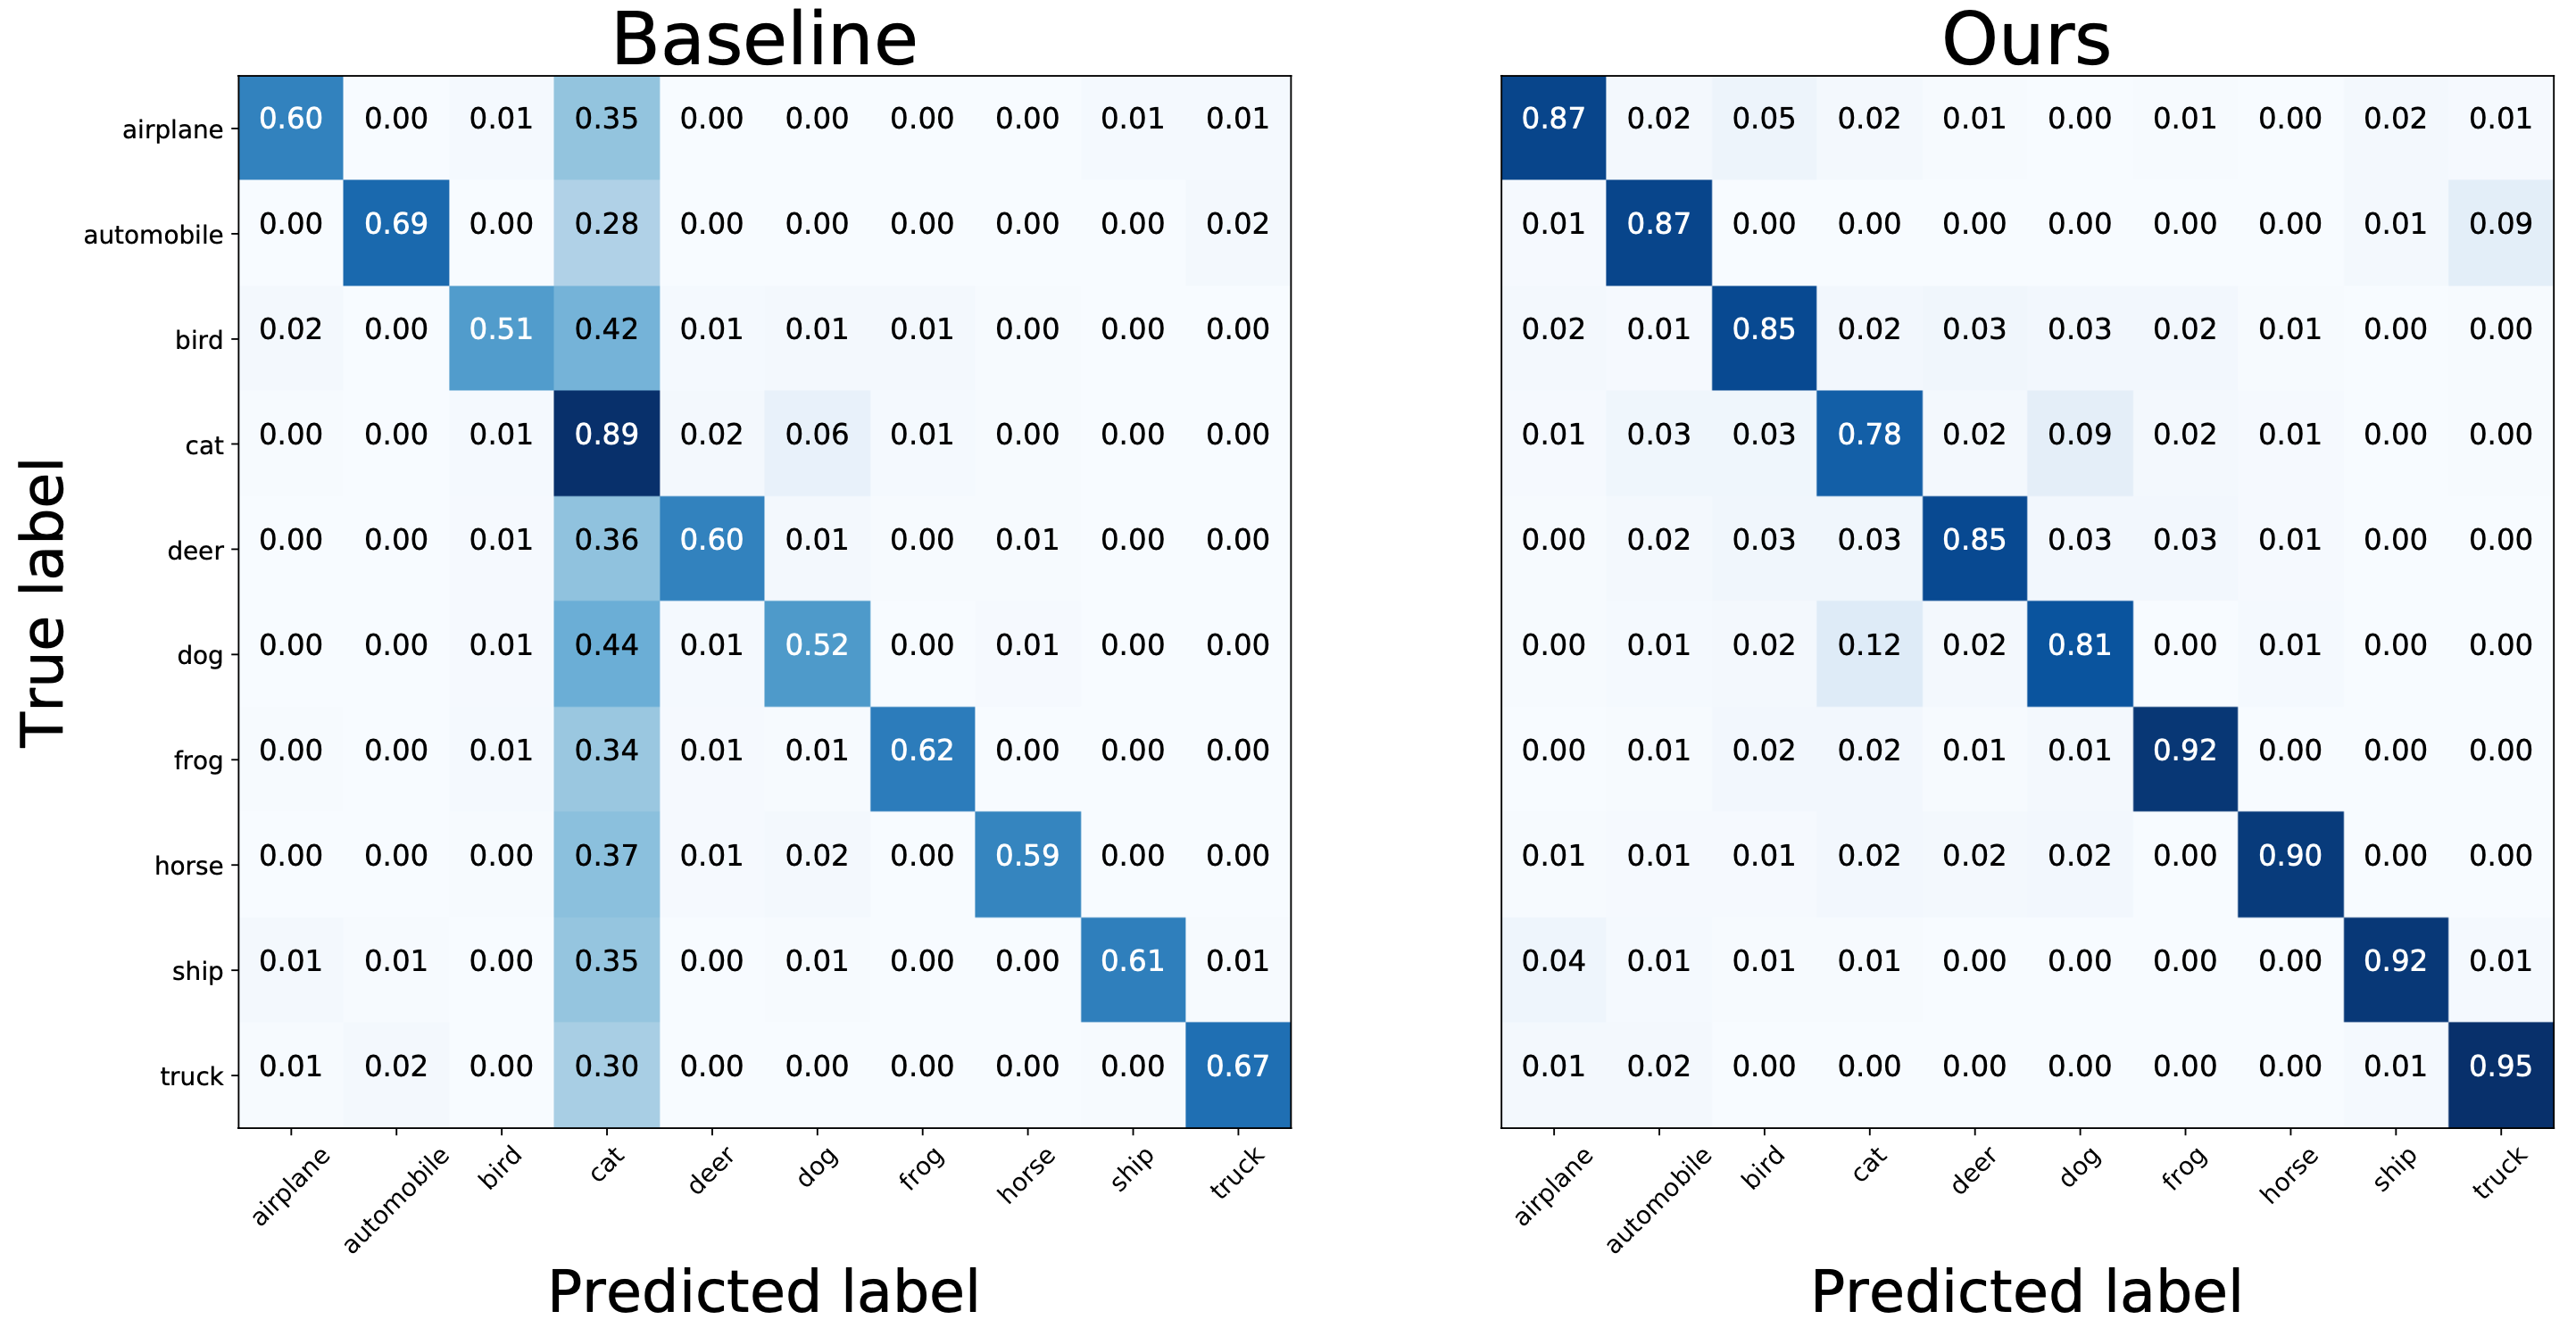
\includegraphics[width=3\columnwidth]{figures/cifar-imbalance-cm.png}
\else
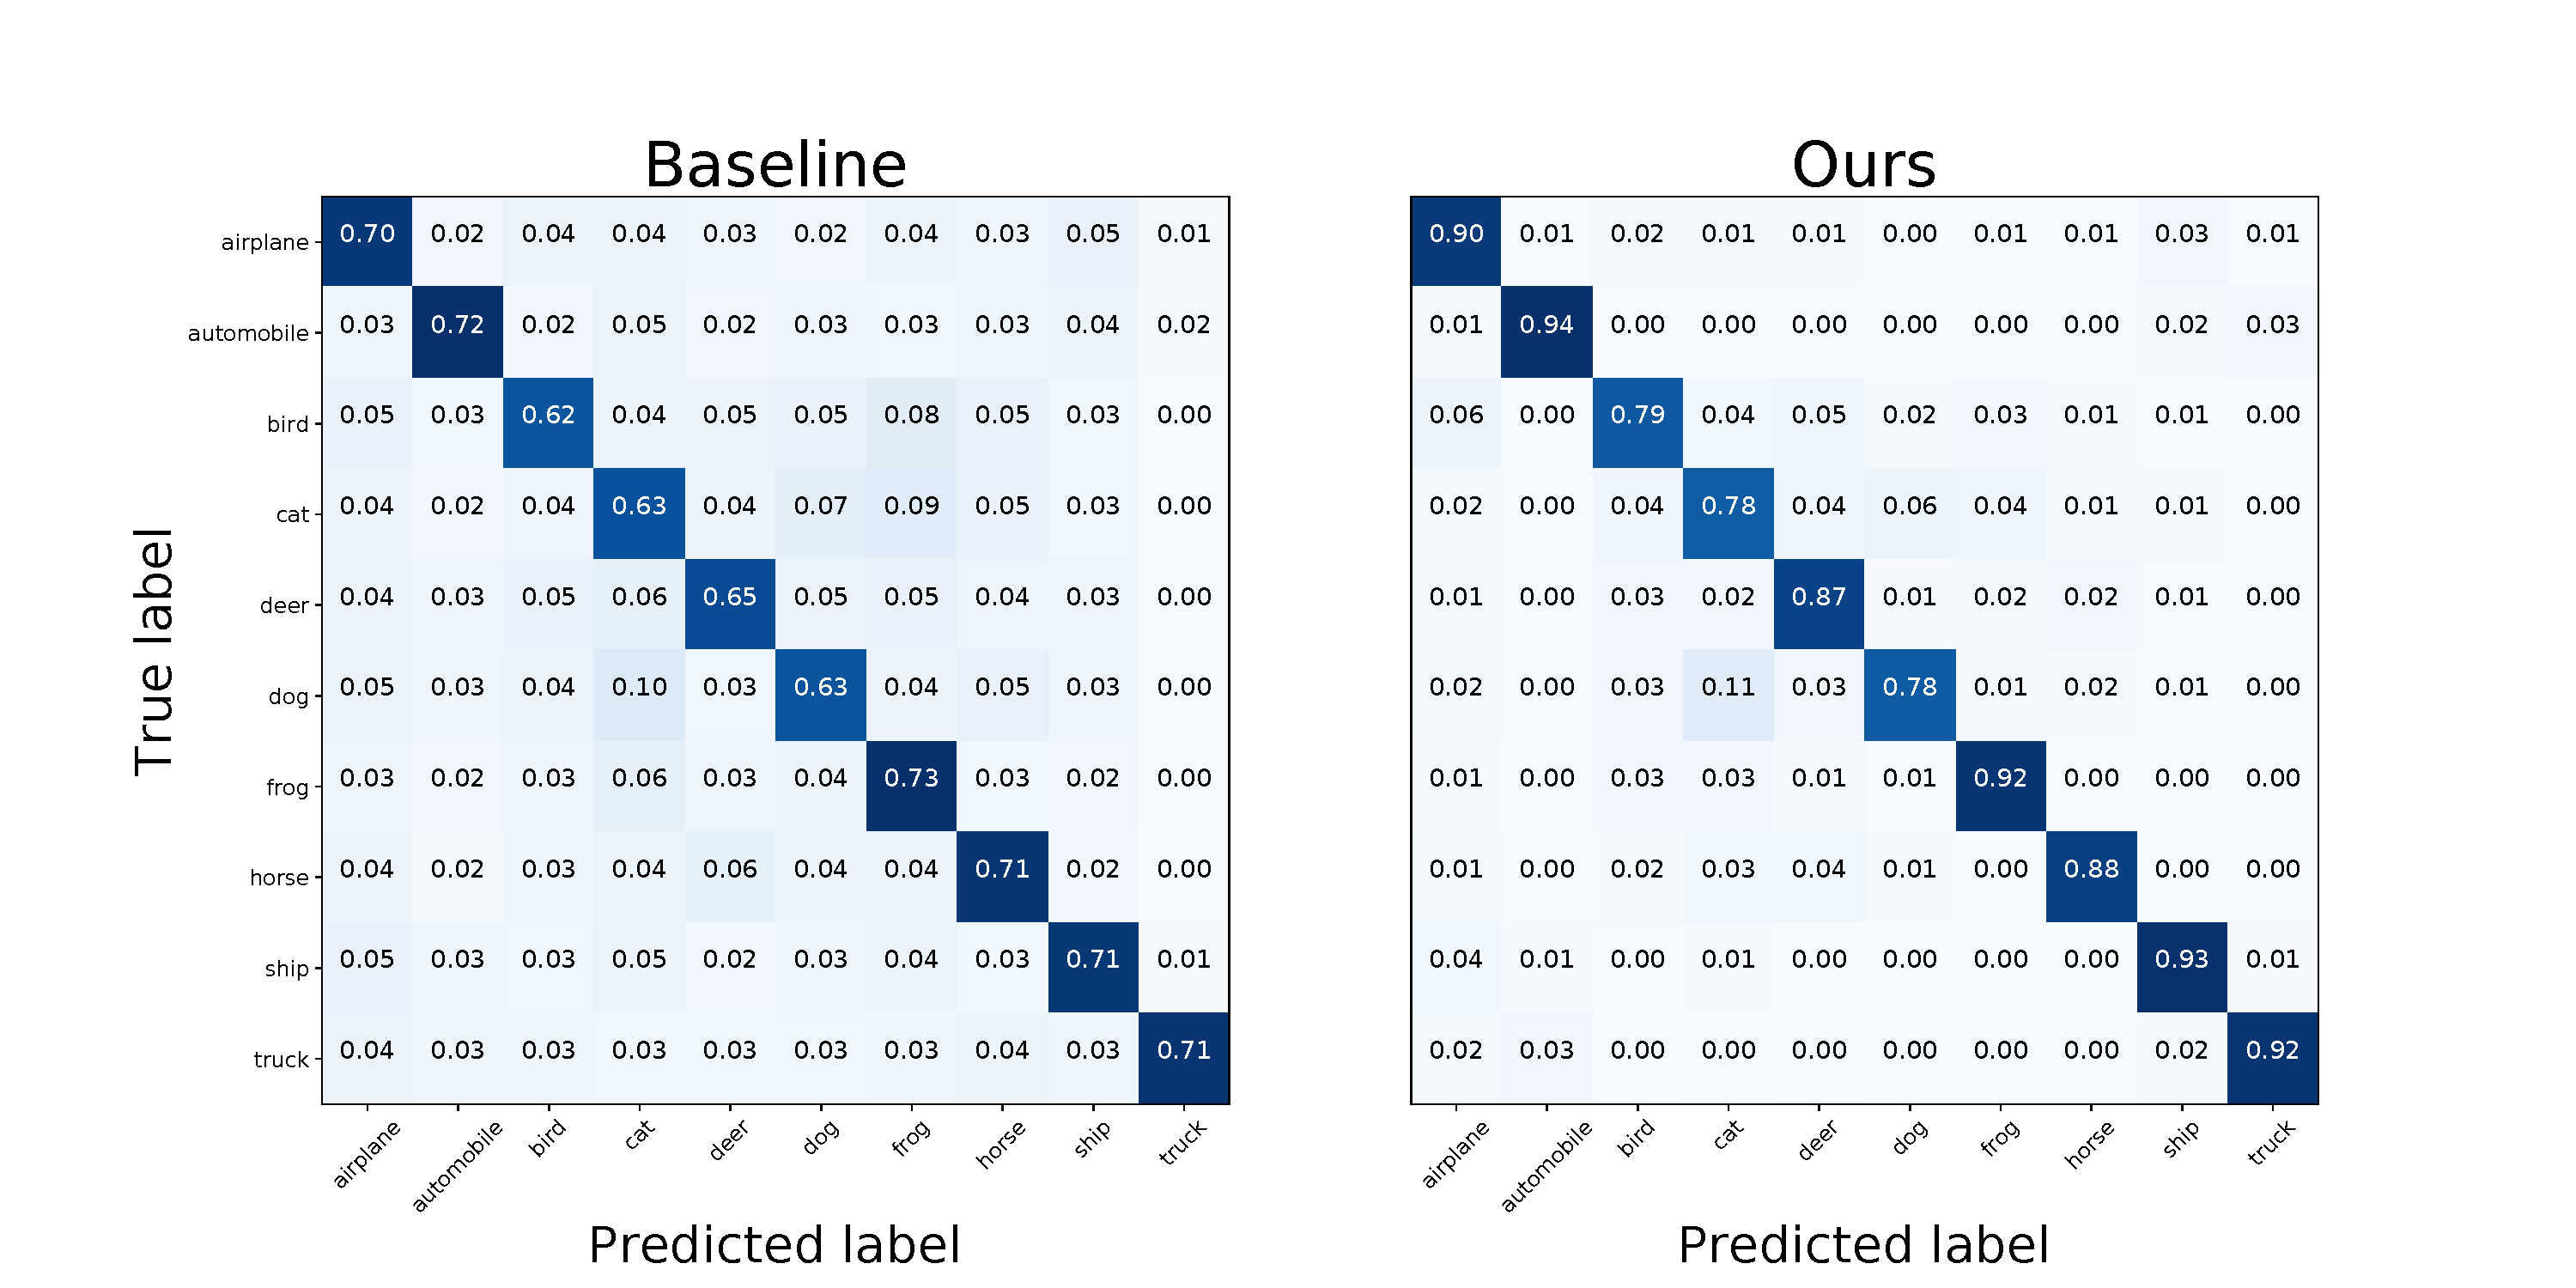
\includegraphics[width=\columnwidth,trim={2.5cm 0 4cm 0},clip]{figures/cifar-noise-cm.pdf}
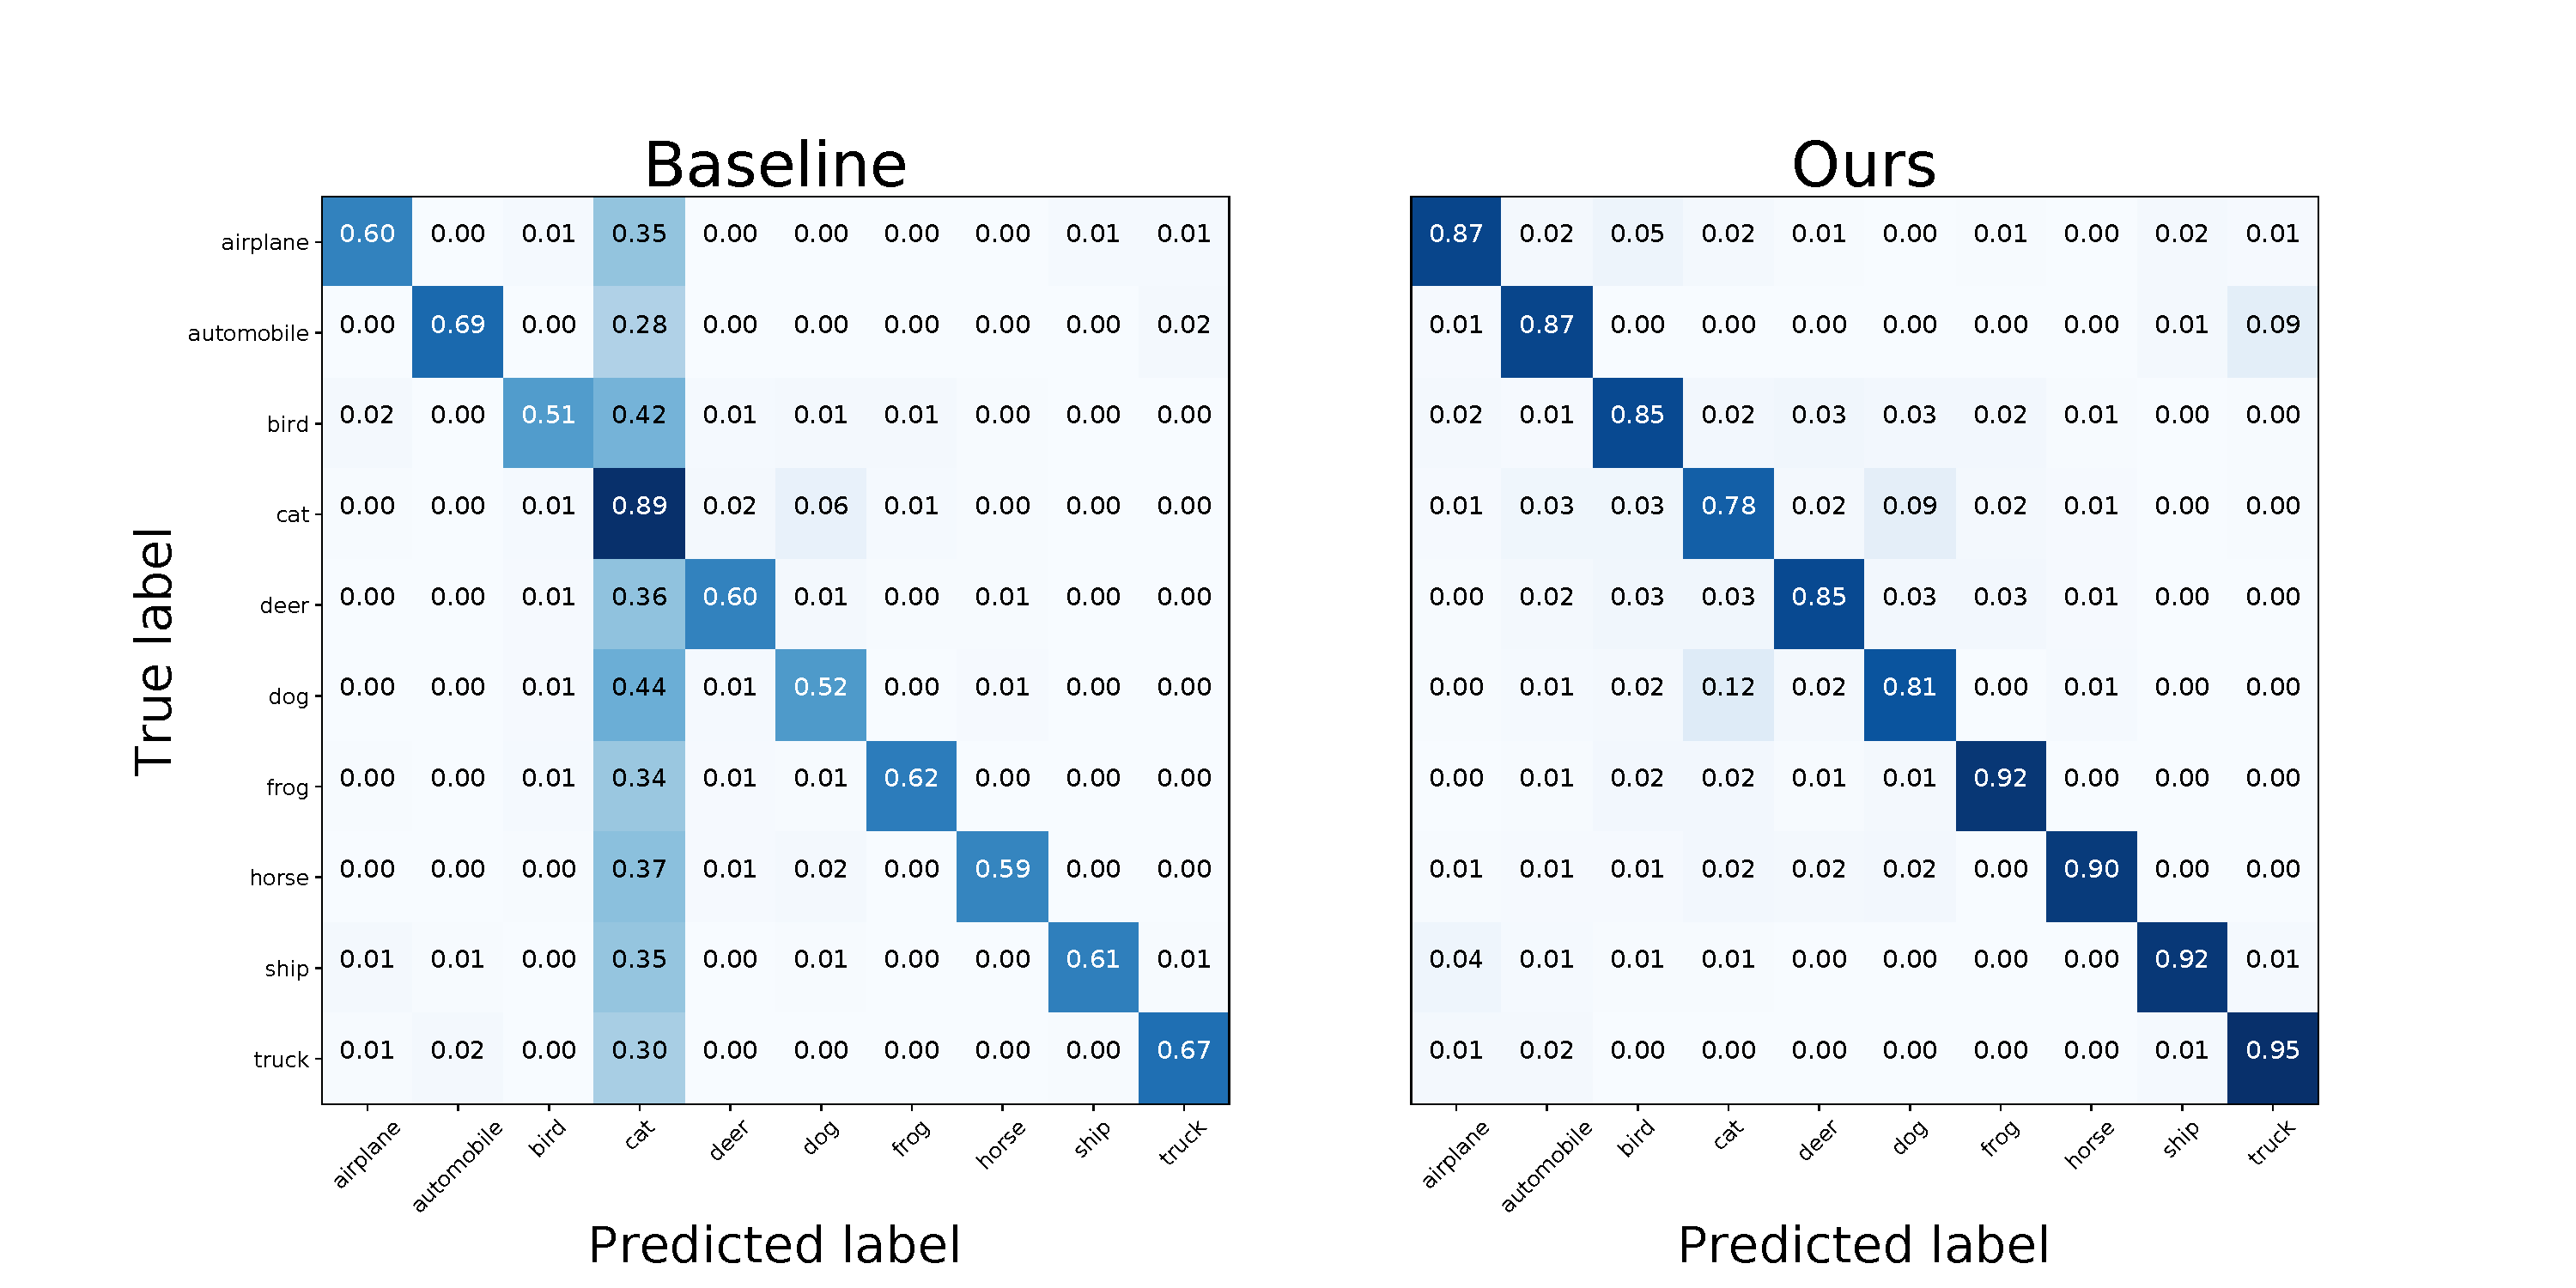
\includegraphics[width=\columnwidth,trim={2.5cm 0 4cm 0},clip]{figures/cifar-imbalance-cm.pdf}
\fi
\vspace{-0.2in}
\iflatexml
\caption{Confusion matrices on CIFAR-10 \textsc{UniformFlip} (left) and \textsc{BackgroundFlip} (right)}
\else
\caption{Confusion matrices on CIFAR-10 \textsc{UniformFlip} (top) and \textsc{BackgroundFlip} (bottom)}
\fi
\label{fig:confusion}
\vspace{-0.1in}
\end{figure}

% !TEX root = ../main.tex
\begin{figure}[h]
\centering
\iflatexml
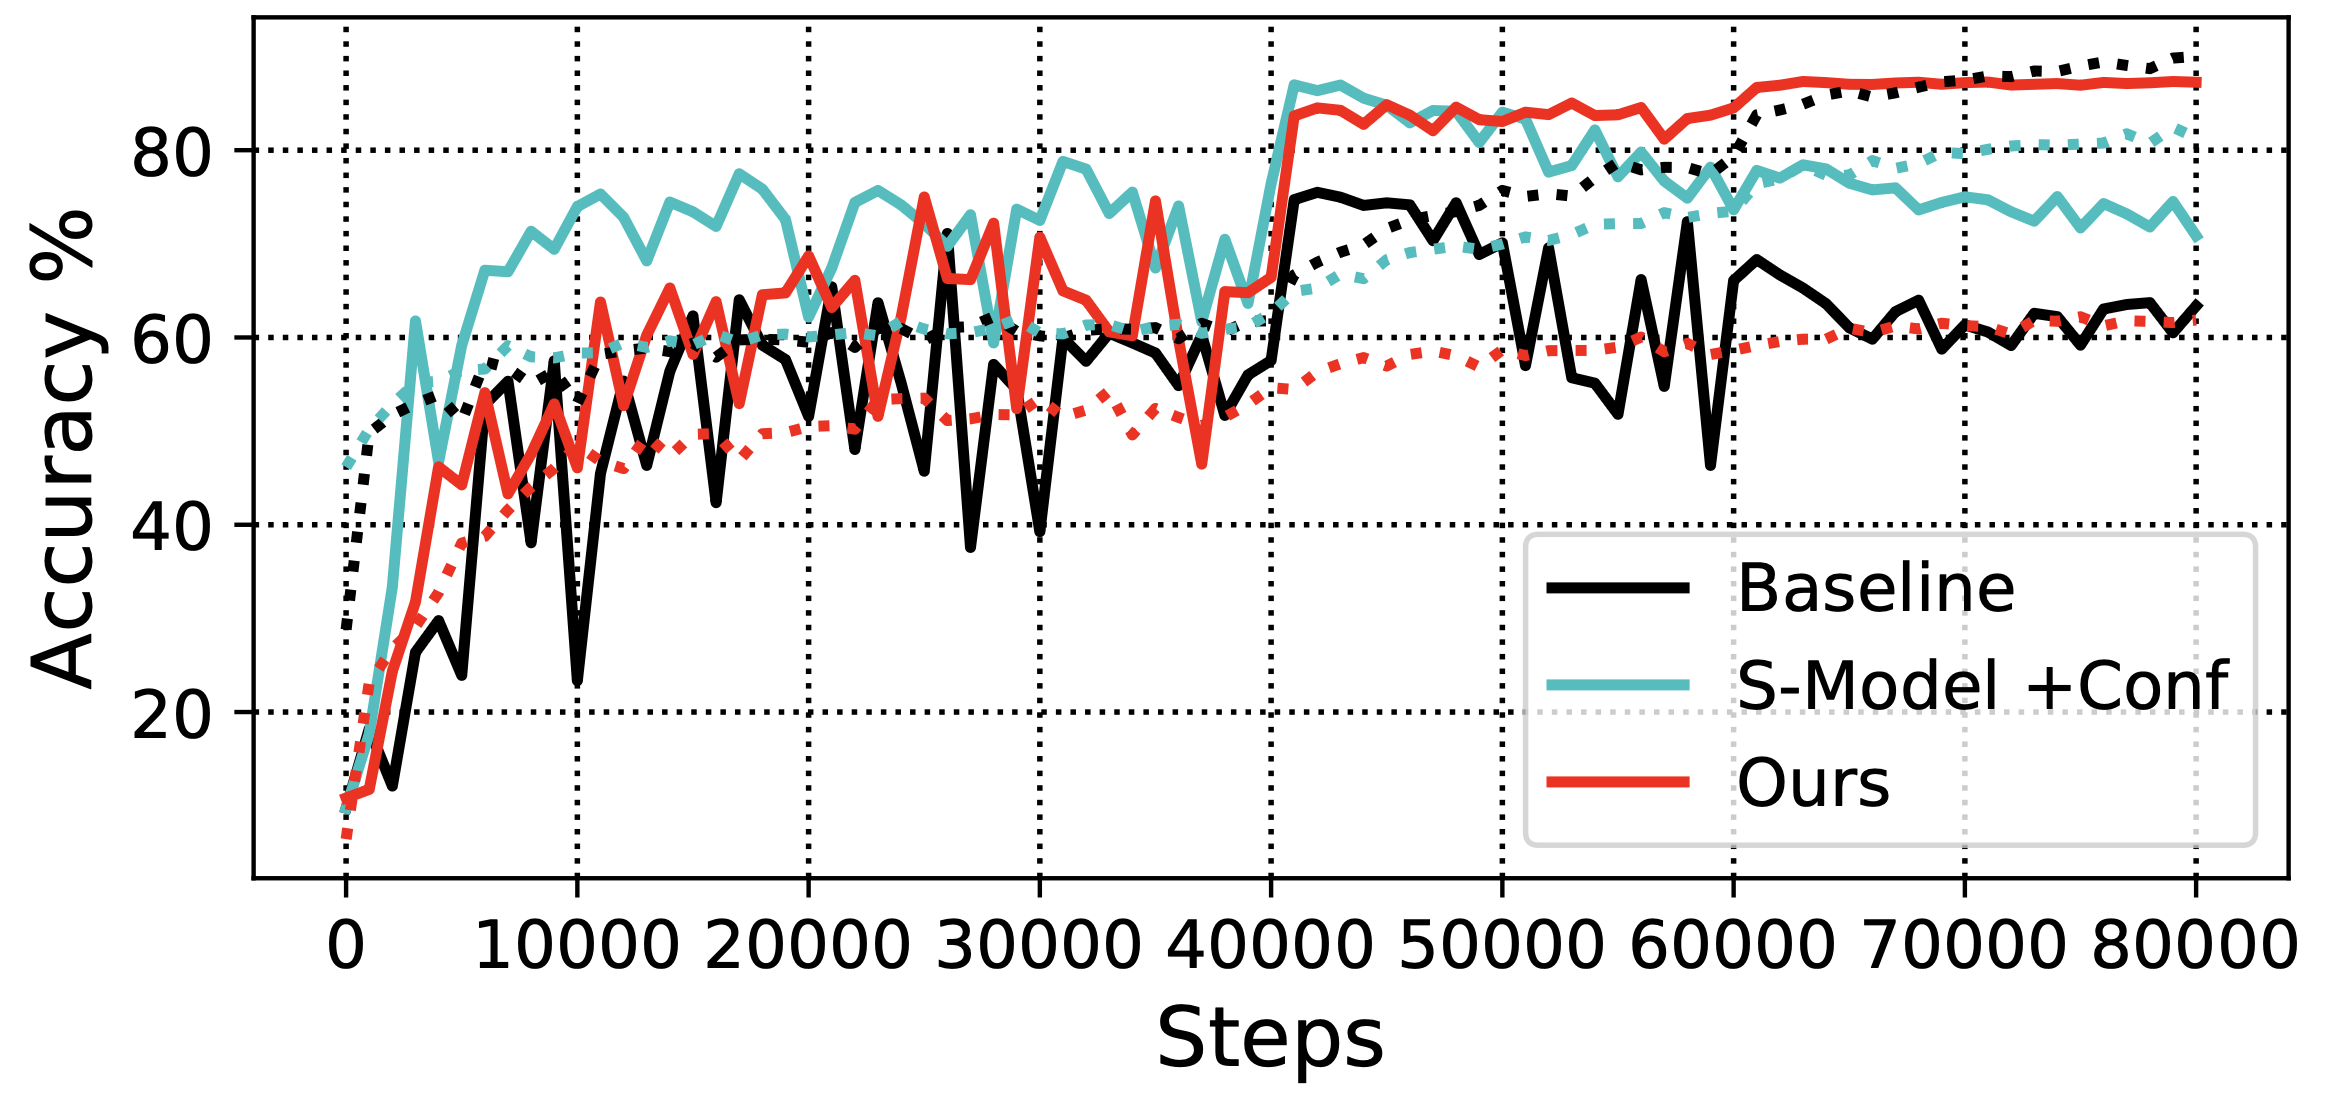
\includegraphics[width=6\columnwidth]{figures/cifar-10-curve.png}
\else
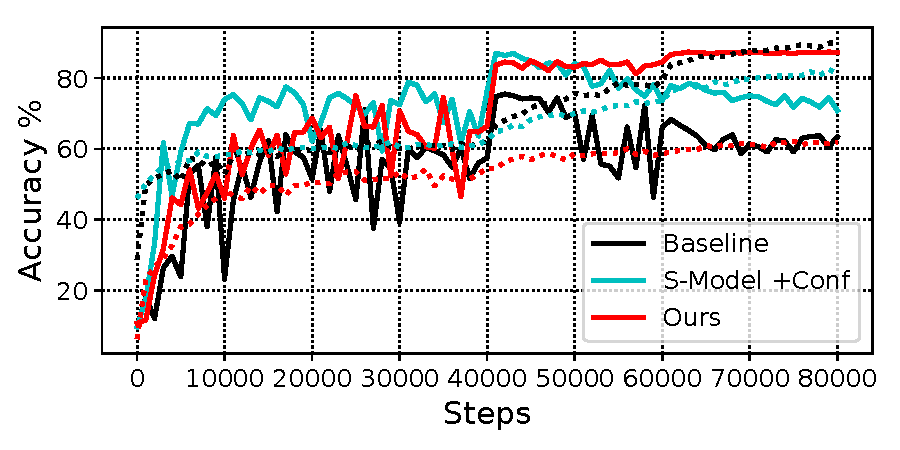
\includegraphics[width=0.9\columnwidth]{figures/cifar-10-curve.pdf}
\fi
\vspace{-0.1in}
\caption{Training curve of a ResNet-32 on CIFAR-10 \textsc{BackgroundFlip} under 40\% noise ratio.
Solid lines denote validation accuracy and dotted lines denote training. Our method is less prone to
label noise overfitting.}
\label{fig:curve}
\vspace{-0.15in}
\end{figure}


\subsection{Results and Discussion}

The first result that draws our attention is that ``Random'' performs surprisingly well on the
\textsc{UniformFlip} benchmark, outperforming all historical methods that we compared. Given that
its performance is comparable with Baseline on \textsc{BackgroundFlip} and MNIST class imbalance, we
hypothesize that random example weights act as a strong regularizer and under which the learning
objective on \textsc{UniformFlip} is still consistent.

Regardless of the strong baseline, our method ranks the top on both \textsc{UniformFlip} and
\textsc{BackgroundFlip}, showing our method is less affected by the changes in the noise type. On
CIFAR-100, our method wins more than 3\% compared to the state-of-the-art method.
\vspace{-0.05in}
\paragraph{Understanding the reweighting mechanism}
It is beneficial to understand how our reweighting algorithm contributes to learning more robust
models during training. First, we use a pre-trained model (trained at half of the total iterations
without learning rate decay) and measure the example weight distribution of a randomly sampled batch
of validation images, which the model has never seen. As shown in the left figure of Figure
\ref{fig:dist}, our model correctly pushes most noisy images to zero weights. Secondly,  we
conditioned the input mini-batch to be a single non-background class and randomly flip 40\% of the
images to the background, and we would like to see how well our model can distinguish clean and
noisy images. As shown in Figure \ref{fig:dist} right, the model is able to reliably detect images
that are flipped to the background class.
\vspace{-0.05in}
\paragraph{Robustness to overfitting noise} Throughout experimentation, we find baseline
models can easily overfit to the noise in the training set. For example, shown in
Table~\ref{tab:backgroundflip}, applying early stopping (``ES'') helps the classification
performance of ``S-Model'' by over 10\% on CIFAR-10. Figure~\ref{fig:confusion} compares the final
confusion matrices of the baseline and the proposed algorithm, where a large proportion of noise
transition probability is cleared in the final prediction. Figure~\ref{fig:curve} shows training
curves on the \textsc{BackgroundFlip} experiments. After the first learning rate decay, both
``Baseline'' and ``S-Model'' quickly degrade their validation performance due to overfitting, while
our model remains the same validation accuracy until termination. Note that here ``S-Model'' knows
the oracle noise ratio in each class, and this information is not available in our method.
\vspace{-0.05in}
\paragraph{Impact of the noise level} We would like to investigate how strongly our method can
perform on a variety of noise levels. Shown in Figure~\ref{fig:level}, our method only drops 6\%
accuracy when the noise ratio increased from 0\% to 50\%; whereas the baseline has dropped more than
40\%. At 0\% noise, our method only slightly underperforms baseline. This is reasonable since we are
optimizing on the validation set, which is strictly a subset of the full training set, and therefore
suffers from its own subsample bias.
\vspace{-0.05in}
\paragraph{Size of the clean validation set} When the size of the clean validation set grows larger,
fine-tuning on the validation set will be a reasonble approach. Here, we make an attempt to explore
the tradeoff and understand when fine-tuning becomes beneficial. Figure~\ref{fig:ft} plots the
classification performance when we varied the size of the clean validation on
\textsc{BackgroundFlip}. Surprisingly, using 15 validation images for all classes only results in a
2\% drop in performance, and the overall classification performance does not grow after having more
than 100 validation images. In comparison, we observe a significant drop in performance when only
fine-tuning on these 15 validation images for the baselines, and the performance catches up around
using 1,000 validation images (100 per class). This phenomenon suggests that in our method the clean
validation acts more like a regularizer rather than a data source for parameter fine-tuning, and
potentially our method can be complementary with fine-tuning based method when the size of the clean
set grows larger.
